% Le système ArcGIS
% Clément Delgrange
% Avril 2018

% Modules generaux
\documentclass[11pt]{article}
\usepackage[utf8]{inputenc}
\usepackage[T1]{fontenc}
\usepackage[francais]{babel} % prise en charge du francais
\usepackage[table]{xcolor} % tableaux
\usepackage{graphicx} % images
\usepackage{float}
\usepackage[font=small]{caption}

% Marges
\usepackage[left=2cm,right=2cm,top=2cm,bottom=2cm]{geometry}

% Personnalisation des titres
\usepackage{titlesec}
\titlespacing{\section}{0em}{4em}{1em}
\titlespacing{\subsection}{0em}{2em}{0em}
\titlespacing{\subsubsection}{0em}{0.5em}{0em}

% Mise en page
\setlength{\parskip}{1.2em}
\renewcommand{\floatpagefraction}{1}

% Couleurs personnalisées
\usepackage{color}
\definecolor{lightgray}{gray}{0.98}
\definecolor{gray}{rgb}{0.6, 0.6, 0.65}
\definecolor{green}{rgb}{0.133, 0.545, 0.133}
\definecolor{blue}{rgb}{0, 0, 1}
\definecolor{red}{rgb}{0.6, 0.1, 0.1}

% Liens hypertextes
\usepackage{hyperref}
\hypersetup{
	colorlinks=true,
	breaklinks=true,
	urlcolor=blue,
	linkcolor=blue,
	pdfborder=000,
	pdftex=true
}

% Mise en forme des codes python
\usepackage{listingsutf8}
\lstset{
	language=python,
	inputencoding=utf8/latin1,
	extendedchars=true,
	keywordstyle=\bfseries\ttfamily\color{blue},
	identifierstyle=\ttfamily,
	commentstyle=\color{gray},
	stringstyle=\ttfamily\color{green},
	showstringspaces=false,
	basicstyle=\footnotesize\ttfamily,
	tabsize=2,
	breaklines=true,
	extendedchars=true,
	xleftmargin=1cm,
	xrightmargin=1cm,
	backgroundcolor=\color{lightgray},
	literate=%
		{é}{{\'{e}}}1
		{è}{{\`{e}}}1
		{ê}{{\^{e}}}1
		{ë}{{\¨{e}}}1
		{û}{{\^{u}}}1
		{ù}{{\`{u}}}1
		{â}{{\^{a}}}1
		{à}{{\`{a}}}1
		{î}{{\^{i}}}1
		{ô}{{\^{o}}}1
		{ç}{{\c{c}}}1
}

% Commandes personnalisées
\newcommand{\bslash}{\texttt{\symbol{92}}}
\newcommand{\action}{$\Rightarrow$ }
\newcommand{\reponse}{
	\begin{tabbing}
	\hspace{2cm}\=\kill
	Réponse \> ............................................................................................ \\
 	\> ............................................................................................
	\end{tabbing}
}

\newenvironment{note}{%
	\begin{tabular}[t t]{c c}
		
\includegraphics{img/tips.png}
		 &
		\begin{minipage}[c]{0.9\linewidth}
			\begin{sffamily}
}{%
			\end{sffamily}
		\end{minipage}
	\end{tabular}
}

\newenvironment{objectifs}{
  \hrule
	\begin{minipage}{0.9\textwidth}
		\vspace{1em}
		\begin{tabular}[t t]{c c}
			
\includegraphics[width=0.1\linewidth]{img/goals.jpg} &
			\begin{minipage}[c]{0.8\linewidth}
				\hspace{2em}\textbf{\large{Objectifs :}} \\
}{
			\end{minipage}
		\end{tabular}
		\vspace{1em}
	\end{minipage}
	\hrule
}

\newcommand{\code}[1]{\lstinline{#1}}

\newenvironment{python}{%
	\begin{lstlisting}
}{%
	\end{lstlisting}
}


%%%%%%%%%%%%%%%%%%%%%%%%%%%%%%%%%
% Infos générales sur le document
%%%%%%%%%%%%%%%%%%%%%%%%%%%%%%%%%
\title{Le système ArcGIS}
\author{Clément Delgrange}
\date{Avril 2018}

% Entetes et pieds de page
\usepackage{fancyhdr}
\pagestyle{fancy}
\fancyhf{}
\renewcommand{\headrulewidth}{0pt}
\makeatletter
\fancyfoot[L]{\@author}
\fancyfoot[C]{-\thepage-}
\fancyfoot[R]{\@title}
\makeatother
\renewcommand{\footrulewidth}{0.5pt}


%%%%%%%%%%%%
%%% Document
%%%%%%%%%%%%
\begin{document}
\parindent=0cm


\begin{titlepage}
\makeatletter
	\begin{sffamily}
		\begin{flushleft}
			% 
\includegraphics{img/logos/ign-logo-ensg.jpg}\\[1.5cm]
		\end{flushleft}
		\begin{flushright}
			% pour mettre une image en haut à droite
		\end{flushright}

		\vspace{4cm}

		\begin{center}
			\hrule
				\vspace{1em}
				{\small \textit{Programmation SIG}}\\
				\vspace{0.5cm}
				{\huge\bfseries \@title}
				\vspace{1cm}
			\hrule

			\vspace{3.5cm}
			%\includegraphics[width=400px]{images/logo_python.png}
			\vspace{5cm}

			\large \textit{\@author}\\
			\small \textit{\@date}
		\end{center}
	\end{sffamily}
\makeatother
\end{titlepage}


\begin{objectifs}
	\begin{itemize}
		\item savoir personnaliser l'affichage d'ArcMap
		\item être capable d'ajouter un plugin à ArcMap
%		\item apprendre à publier un service sur un serveur ArcGIS
		\item savoir connecter des applications Esri à des ressources en ligne
		\item créer une application web SIG simple à l'aide des technologies Esri
	\end{itemize}
\end{objectifs}


\section*{Préalables}

Au cours de ce TD, nous allons publier sur ArcGIS Online des données localisées autour de la cité Descartes pour ensuite créer une application web SIG permettant de les visualiser.
Avant de commencer le travail de publication, nous utiliserons ArcMap pour effectuer un contrôle minimal des données sources à notre disposition.

\action Rendez-vous sur \url{arcgis.com} pour vous créer un compte personnel ArcGIS Online si vous n'en possédez pas déjà un.

Les données initiales se trouvent sur le \href{https://github.com/ClementDelgrange/Cours_programmation_SIG/tree/master/data}{dépôt github du cours}.

\action Copiez-les sur votre poste dans \textit{D:\textbackslash{}ProgSIG\textbackslash{}TD3\textbackslash{}Data}.



\section{Préparation des données}

\action Dans ArcMap, créez un nouveau document \textit{TD3.mxd} que vous enregistrerez dans \textit{D:\textbackslash{}ProgSIG\textbackslash{}TD3}.

Nous allons commencer par ajouter une connexion au dossier dans lequel les données ont été copiées pour pouvoir les utiliser plus facilement dans ArcMap.

\action Dans l'onglet ArcCatalog, cliquez sur \textbf{Ajouter une connexion à un dossier}.
\begin{figure}[H]
	\center 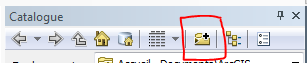
\includegraphics{img/cours3/am_ajouter_connexion_dossier.png}
\end{figure}

\action Pointez vers le dossier local où se trouvent vos données pour le TD et faites \textbf{OK}.

Le répertoire \textit{data} avec les trois shapefiles copiés apparaît dans la liste des dossiers connectés :
\begin{figure}[H]
	\center 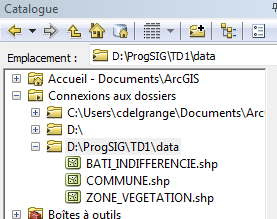
\includegraphics{img/cours3/am_ajouter_connexion_dossier_ok.png}
\end{figure}

\action Ajoutez votre document les shapefiles VEGETATION.shp, BATI\_INDIFERRENCIE.shp et COMMUNE.shp.
\begin{figure}[H]
	\center 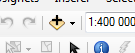
\includegraphics{img/cours3/am_ajouter_donnees.png}
\end{figure}

Nous allons également ajouter à notre document un fond de carte OpenStreetMap hébergé sur les serveurs d'Esri.

\action Dans \textbf{Fichier > Ajouter des données > Ajouter un fond de carte}, sélectionnez le fond de carte OpenStreetMap.

\begin{note}
Vous pouvez aussi utiliser le bouton \textbf{Ajouter des données} de la barre d'outils standards.
\begin{figure}[H]
	\center 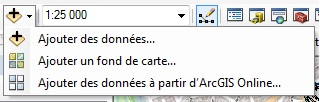
\includegraphics{img/cours3/am_ajouter_fond_carte.jpg} \\
\end{figure}
\end{note}

\vspace{2em}
Nous voulons nous assurer que nos données de départ ne présentent pas trop d'incohérences. Nous allons pour cela effectuer deux types de contrôles :
\begin{itemize}
  \item vérifier de manière exhaustive la validité des géométries;
	\item vérifier de manière exhaustive qu'il n'y a pas d'entités en double;
	\item de manière plus qualitative, s'assurer qu'il ne manque pas de bâtiment.
\end{itemize}

Pour le premier contrôle, nous utiliserons le \textit{Vérifier les géométries}, du \textit{Jeu d'outils Entités} (dans les ArcToolbox).

\action Après avoir identifé l'outil, exécutez le sur chacune des couches chargées. Corrigez les problèmes si vous en trouvez.

Pour le second contrôle, nous nous aiderons d'une extension \textit{SelectStackedFeatureAddIn}, disponible dans les données sources que vous avez copiées sur votre poste.

Une extension ArcMap se présente sous la forme d'un fichier \textit{.esriAddIn}.
Derrière cette extension se cache juste un dossier compressé (.zip) contenant
\begin{itemize}
  \item un fichier de configuration décrivant la structure de l'extension;
  \item quelques images pour les icônes de l'extension;
  \item divers exécutables.
\end{itemize}
Vous vous en convaincrez en en décompressant une (clic droit > 7-zip > Extraire les fichiers).
\begin{figure}[H]
	\center 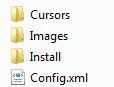
\includegraphics{img/cours3/contenu_addin.jpg} \\
\end{figure}

\action Double-cliquez sur le fichier \textit{SelectStackedFeatures.esriAddIn} pour installer l'extension.
\begin{figure}[H]
	\center 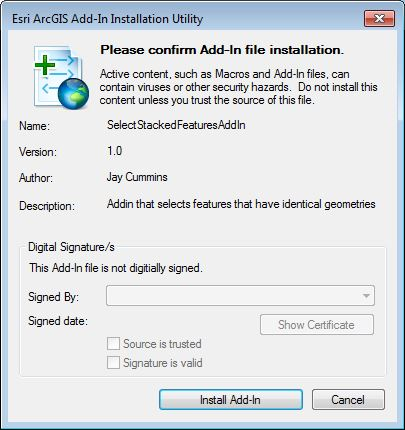
\includegraphics[width=0.37\textwidth]{img/cours3/install_addin.jpg} \\
\end{figure}

\action Relancez ArcMap une fois l'installation terminée pour que l'extension soit prise en compte.

En allant dans le menu \textbf{Personnaliser > Gestionnaire de compléments}, vous pouvez constater que l'extension est bien reconnue par ArcMap.
\begin{figure}[H]
	\center 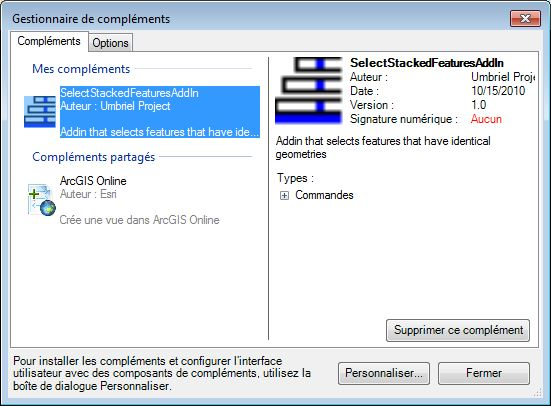
\includegraphics[width=0.5\textwidth]{img/cours3/am_gestionnaire_complements.jpg} \\
\end{figure}

\begin{note}
A chaque ouverture d'ArcMap, un ensemble de répertoires sont scannés pour voir si des extensions y sont présentes. Par défaut, seul le répertoire C:\textbackslash{}Users\textbackslash{}<user>\textbackslash{}Documents\textbackslash{}ArcGIS\textbackslash{}AddIns\textbackslash{}Desktop10.X est regardé. L'installation d'une extension comme nous l'avons fait n'est en fait qu'une simple copie du fichier \textit{.esriaddin} vers ce dossier.

Mais il est tout à fait possible d'indiquer à ArcMap que d'autres répertoires doivent êtres scannés. Cela sera notamment utile pour qu'une même extension soit installée par plusieurs utilisateurs. Dans le menu \textbf{Personnaliser > Gestionnaire de compléments}, onglet \textbf{Options}, vous pouvez paramétrer les répertoires scannés au démarrage de l'application.

Vous pouvez par exemple ajouter le répertoire D:\textbackslash{}ProgSIG.
\begin{figure}[H]
	\center 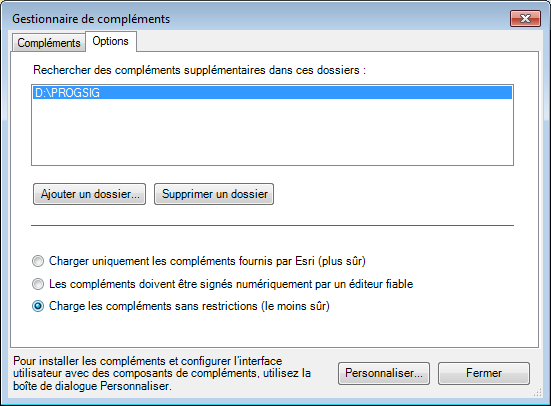
\includegraphics[width=0.5\textwidth]{img/cours3/am_gestionnaire_complements_options.png} \\
\end{figure}

Pour installer des extensions, il suffira alors de copier le fichier \textit{.esriAddIn} dans l'un des répertoires scannés.
\end{note}

Nous allons maintenant créer une nouvelle barre d'outils dans laquelle nous insèrerons un bouton permettant d'exécuter l'extension \textit{SelectStackedFeatureAddIn}.

\action Dans le menu \textbf{Personnaliser} ouvrez la fenêtre \textbf{Mode personnalisation...} et cliquez sur \textbf{Nouveau} pour créer une nouvelle barre d'outils.
\begin{figure}[H]
	\center 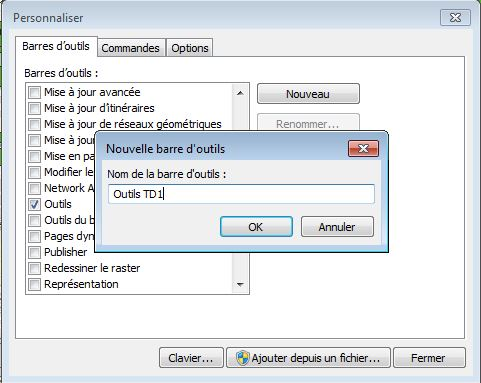
\includegraphics[width=0.5\textwidth]{img/cours3/am_fenetre_personnaliser.png} \\
\end{figure}

\action Passez à l'onglet \textbf{Commandes} pour rechercher la commande liée à l'extension \textit{SelectStackedFeatureAddIn} (soit via l'entrée \textit{Umbriel}, soit en effectuant une recherche \textit{select stacked}).
\begin{figure}[H]
	\center 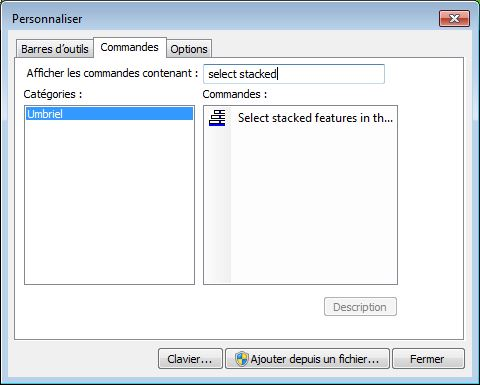
\includegraphics[width=0.5\textwidth]{img/cours3/am_fenetre_personnaliser-2.png} \\
\end{figure}

\action Glissez-déposez la commande sur votre barre d'outils pour l'y ajouter.

L'extension est maintenant prête à être à être utilisée.
\begin{figure}[H]
	\center 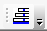
\includegraphics{img/cours3/am_detection_doublons.png} \\
\end{figure}

\action Lancez la détection des doublons sur chacune des trois couches et corrigez les problèmes si l'outil en détecte (\textit{passer en mode édition, supprimer l'entité, etc.}).

\begin{note}
Les modifications de l'interface (ajout / modification / suppression / réorganisation de barres d'outils) sont attachées au document ArcMap (le mxd). Créer un nouveau document a pour effet de réinitialiser complètement l'interface.

Pour que des modifications soient permanentes, c'est à dire conservée lors de la création de nouveau document, la solution consiste à intervenir sur le modèle de document (fichier .mxt) qui se trouve dans le répertoire \textit{C:\textbackslash{}Users\textbackslash{}<user>\textbackslash{}AppData\textbackslash{}Roaming\textbackslash{}ESRI\textbackslash{}Desktop10.X\textbackslash{}ArcMap\textbackslash{}Templates}.
\end{note}

Une fois les corrections nécessaires effectuées, vous pouvez passer à la deuxième phase des contrôles : l'exhaustivité des bâtiments. Nous comparerons la BD Topo à notre disposition à une couche à priori plus récente : le fond de carte OpenStreetMap. En cas de différence constatée, nous naviguerons dans Street view pour trancher\footnote{La BD Topo est une base de données topographique produite par l'IGN. OpenStreetMap est un projet ayant pour but de constituer une base de données géographique libre du monde. Google Street View est un service de navigation virtuelle lancé par Google. Notre démarche, consistant à contrôler le BD Topo à partir de données OpenStreetMap ou Google, n'a bien entendu aucun sens en terme de production de données. Il s'agit uniquement pour nous de manipuler diverses données géographiques.}.

Le contrôle ne sera pas exhaustif : nous nous concentrerons uniquement sur de petites zones (par exemple les bâtiments autour de l'ENSG).

\action Installez l'extension \textit{StreetViewAddin} qui intègre un module Google StreetView à ArcMap et ajoutez la commande à votre barre d'outils.

\action Vérifiez que les bâtiments d'OpenStreetMap sont identiques à ceux de la BD Topo et utiliser l'extension Street View en cas de besoin pour déterminer si une correction doit être apportée. Complétez la BD Topo si nécessaire.

A ce stade, nous considérons que nos données de base sont correctes et qu'elles peuvent être publiées sur un serveur SIG en ligne.



\section{Publication sur ArcGIS Online}

ArcGIS Online est une plateforme offrant des services web d'accès, de traitements et de diffusion de données géographiques. Elle peut être utilisée pour gérer des données géographiques sans avoir besoin d'installer un serveur, ce que nous illustrerons dans un premier temps. Elle intervient également parfois en complément d'un ArcGIS Entreprise pour diffuser plus facilement des services.

\action Dans un navigateur web, rendez-vous sur \url{arcgis.com} et connectez-vous à votre compte.

Une bannière est présente en haut des pages du site ArcGIS Online et permet d'accéder aux différentes fonctionnalités.
\begin{figure}[H]
	\center 
\includegraphics[width=0.9\textwidth]{img/cours3/ago_banniere.jpg} \\
\end{figure}

Les pages qui pourrons nous intéresser seront :
\begin{itemize}
	\item \textbf{Bibliothèque} liste un ensemble de ressources publiques (fonds de plan par exemple);
	\item \textbf{Carte} ouvre une visionneuse de cartes;
	\item \textbf{Contenu} permet d'accéder aux différents contenus (services, applications web SIG, etc.) sur lesquels vous avez des droits.
\end{itemize}

\vspace{1em}

\action Cliquez sur \textbf{Carte} dans la bannière supérieure pour ouvrir la visionneuse de cartes.

Nous souhaitons dans un premier temps ajouter le shapefile BATI\_INDIFFERENCIE à la carte. Les shapefile doivent être zippés avant d'être ajoutés à la visionneuse de carte.

\begin{note}
Le shapefile est un format de fichier développé initialement par Esri et qui s'est imposé comme un standard dans le monde des SIG. Le terme de \textit{shapefile} est trompeur puisque le format consiste en une collection de fichiers d'extensions différentes, mais portant le même nom est stockés dans le même répertoire. Trois fichiers sont obligatoire pour constituer un shapefile valide :
\begin{itemize}
	\item \code{.shp} : fichier principal décrivant les entités enregistrées (type de géométrie, géométrie de l'entité, rectangle englobant, etc.);
	\item \code{.dbf} : table dBase contenant les attributs des entités géométriques décrites dans le \code{.shp};
	\item \code{.shx} : fichier d'index permettant de retrouver plus rapidement une entité dans le \code{.shp}.
\end{itemize}
D'autres fichier peuvent apporter des informations complémentaires :
\begin{itemize}
	\item \code{.prj} : fichier ne contenant qu'une seule ligne décrivant au format WKT le système de projection utilisé pour représenter les entités;
	\item \code{.sbx} et \code{.sbn}: fichiers d'index spatial, utilisés par les applications Esri uniquement, pour optimiser les requêtes spatiales;
	\item \code{.cpg} : utilisé pour préciser le système d'encodage utilisé dans le \code{.dbf};
	\item \code{.shp.xml} : métadonnées sur le shapefile au format XML;
	\item etc.
\end{itemize}
Notons pour refermer cette parenthèse sur le format shapefile qu'il ne permet pas de stocker d'informations sur la topologie, ni de mélanger des géométries de type différent et est limité en volume (2 Go).
\end{note}

\action Quels fichiers du shapefile serons nécessaires pour l'ajout dans ArcGIS Online ?

\reponse

\action Dans l'explorateur de fichier de windows, zippez les fichiers du shapefile BATI\_INDIFFERENCIE, puis retournez sur la visionneuse de carte ArcGIS Online et ajoutez le shapefile compressé à la carte via le menu \textbf{Ajouter > Ajouter une couche à partir d'un fichier}.
\begin{figure}[H]
	\center 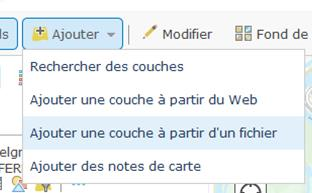
\includegraphics{img/cours3/ago_ajout_couche.jpg} \\
\end{figure}

La classe d'entités s'ajoute au fond de plan pour un rendu assez similaire à ce que nous avions dans ArcMap (vous avez la possibilité de modifier le fond de plan).

Nous allons enregistrer la carte de la visionneuse pour pouvoir nous en resservir par la suite.

\action Cliquez sur le bouton \textbf{Enregistrer > Enregistrer}.
\begin{figure}[H]
	\center 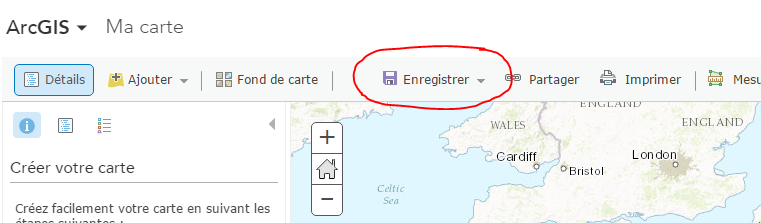
\includegraphics[width=0.6\textwidth]{img/cours3/ago_enregistrer_carte.png} \\
\end{figure}

\action Nommez votre carte \textit{BATI\_DESCARTES} et ajouter une balise \textit{ENSG}.
\begin{figure}[H]
	\center 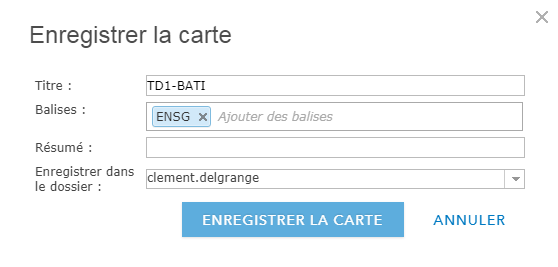
\includegraphics[width=0.5\textwidth]{img/cours3/ago_enregistrer_carte-2.png} \\
\end{figure}

Vous pouvez alors vous rendre sur la page \textbf{Contenu} pour constater que la Web Map a bien été enregistrée.
\begin{figure}[H]
	\center 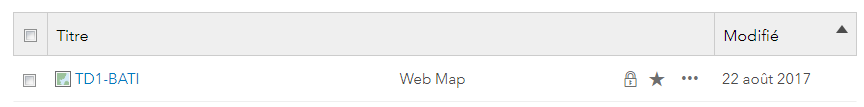
\includegraphics[width=0.7\textwidth]{img/cours3/ago_web_map_ok.png} \\
\end{figure}

\action Dans la zone en haut à gauche, effectuez une recherche avec le mot clé \textit{ENSG}.
\begin{figure}[H]
	\center 
\includegraphics[width=0.4\textwidth]{img/cours3/ago_recherche.png} \\
\end{figure}

Vous devez constater que seul votre ressource est visible. Celles de vos camarades ne seront présentes que s'ils décident de les partager.

\action Si vous le souhaitez, partagez votre carte en la sélectionnant dans vos contenus et en cliquant que \textbf{Partager}, puis \textbf{Tous le monde (public)}.
\begin{figure}[H]
	\center 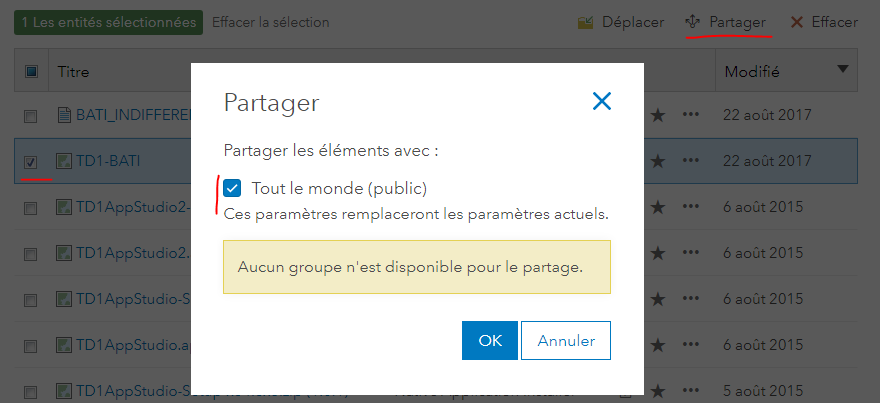
\includegraphics[width=0.65\textwidth]{img/cours3/ago_partager_carte.png} \\
\end{figure}

Relancez la recherche pour constater que vous obtenez plus de résultats.

\begin{note}
Une carte partagée de cette manière sur ArcGIS Online pourra être consultée par l'ensemble des utilisateurs de la plateforme. Mais ils devront effectuer une copie dans leur contenu personnel pour pouvoir la modifier.
\end{note}

Si vous avez partagé votre carte, annulez maintenant ce partage (sélection de la ressource > \textbf{Partager}, puis décochez la case \textbf{Tous le monde}).

\begin{note}
La visionneuse de documents d'ArcGIS Online offre plus de possibilités que ce à quoi nous nous sommes limités ici : création/édition d'entités, modification de leur symbologie... En revanche, elle ne permet pas d'exécuter d'outils de géotraitements. Pour utiliser des géotraitements, nous n'aurons d'autres choix que de revenir dans une application bureautique ou effectuer des développements pour les rendre accessibles via une application web SIG.
\end{note}

%Intéressons nous maintenant à l'utilisation de services publiés sur un serveur ArcGIS.
%
%\action Créez une nouvelle carte
%
%\action Ajoutez un service web : \textbf{Ajouter > Ajouter une couche à partir du web}
%
%\action Sélectionnez alors \textit{Service Web ArcGIS Server} et indiquez l'URL du service de carte publié lors de la première partie du TD.
%\begin{figure}[H]
%	\center 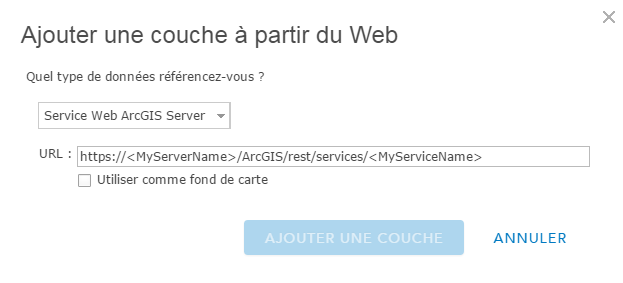
\includegraphics[width=0.5\textwidth]{img/cours3/ago_ajouter_service_web.png} \\
%\end{figure}
%
%\action De la même manière que précédemment, enregistrez et partagez votre carte (nom \textit{TD1}, balises \textit{TD1} et \textit{ENSG}).
%
%Ces étapes ont permis de partager un service web qui était déjà publié sur un ArcGIS for Server.
%
%\action Quels sont selon vous les intérêts d'une telle manipulation ?
%
%\reponse



\section{Utilisation de ressources en ligne}
Dans cette partie, nous explorerons des manières de visualiser et utiliser des ressources publiées sur ArcGIS Online.

\subsection{Dans ArcMap}
\action Dans ArcMap, créez un nouveau document.

\action Ouvrez la  boîte de dialogue ArcGIS Online (menu \textbf{Fichier > ArcGIS Online}).

\action Effectuez une recherche à l'aide du mot clé \textit{ENSG} dans le but d'ajouter votre carte \textit{BATI\_DESCARTES} au document ArcMap.

\action Le résultat est-il celui attendu ? Pourquoi ?

\reponse

\action Connectez-vous maintenant à votre compte ArcGIS Online (\textbf{Fichier > Se connecter...}) et relancez la recherche.

\action Ajoutez alors votre carte \textit{BATI\_DESCARTES} au document ArcMap en cliquant sur \textbf{Ouvrir}.
\begin{figure}[H]
	\center 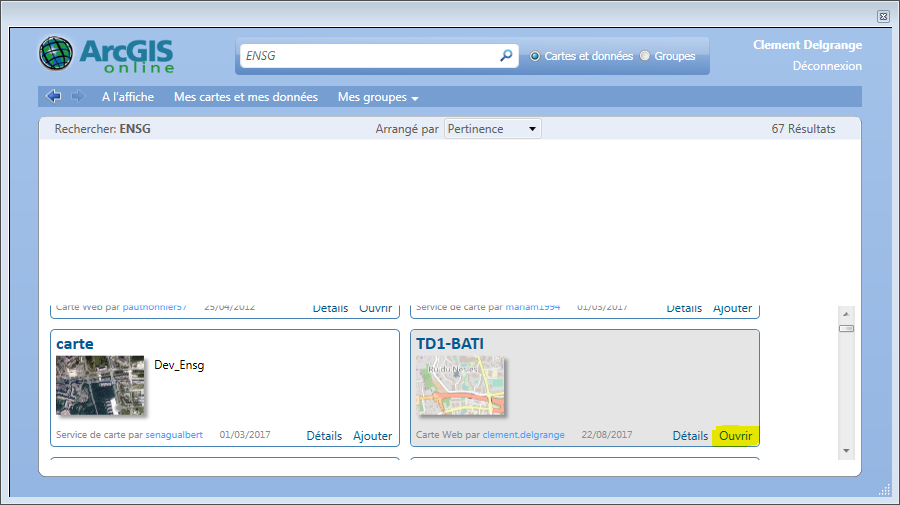
\includegraphics[width=0.6\textwidth]{img/cours3/am_ouvrir_service_ago.png} \\
\end{figure}

Le chargement de cette carte ArcGIS Online a ajouté à notre document des données d'origine variées :
\begin{itemize}
	\item une classe d'entités publiée sur ArcGIS Online
%	\item une classe d'entités publiée sur ArcGIS for Server et routée sur ArcGIS Online
	\item un fond de carte hébergé sur ArcGIS Online
\end{itemize}

%L'étape suivante consiste à charger dans ArcMap le flux WMS que l'on a activé en publiant notre ressource sur ArcGIS for Server.
%
%\action Retrouvez tout d'abord l'URL de ce flux WMS :
%
%\reponse
%
%\action Dans le catalogue d'ArcMap, sous serveur SIG, \textbf{Ajouter un serveur WMS}.
%\begin{figure}[H]
%	\center 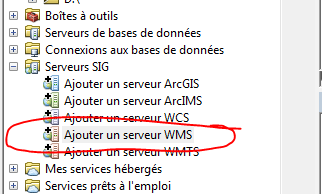
\includegraphics{img/cours3/am_ajout_wms-1.png} \\
%\end{figure}
%
%\action Indiquez l'URL de votre flux WMS, vérifiez les couches disponibles et validez.
%\begin{figure}[H]
%	\center 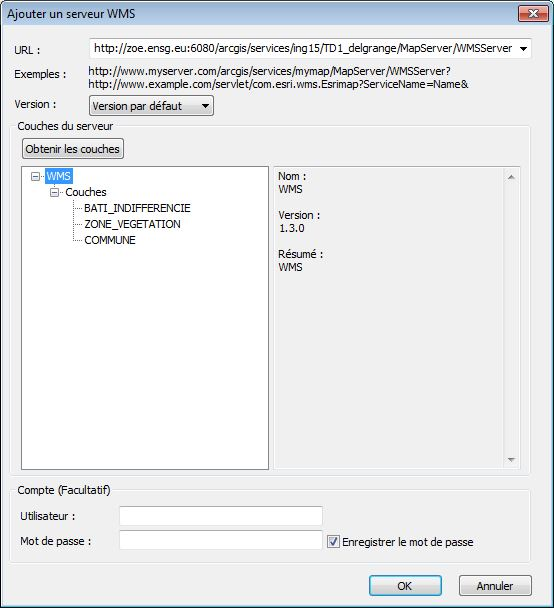
\includegraphics[width=0.5\textwidth]{img/cours3/am_ajout_wms-2.jpg} \\
%\end{figure}
%
%Les couches apparaissent dans le catalogue d'ArcMap.
%
%\action Il ne reste plus qu'à glisser vos couches WMS dans le document pour les y ajouter.
%
%\action Visualisez et interrogez les données. Quelle constatation pouvez-vous faire ?
%
%\reponse


\subsection{Création d'une application web SIG}
Dans le paragraphe précédent, nous avons consommé des services ArcGIS depuis l'application bureautique ArcMap. Cette solution présente un inconvénient majeur : il est nécessaire de disposer d'ArcMap et de savoir s'en servir un minimum! Aujourd'hui les utilisateurs de données géographiques ne sont plus nécessairement des professionnels de la géomatique. Une manière élégante pour leur faciliter l'accès aux données géographiques sera de présenter ces données et les fonctionnalités dont ils ont besoin via une application web SIG.

La couche \textit{Export\_Bati} est présente sur votre carte \textit{BATI\_DESCARTES}, mais nulle part ailleurs. Nous allons commencer par l'enregistrer en tant que couche pour que quelqu'un puisse la retrouver.

\action Dans la visionneuse de carte, ouvrez les propriétés de la couche \textit{Export\_Bati} et sélectionnez \textbf{Enregistrer la couche} au bas du menu.
\begin{figure}[H]
	\center 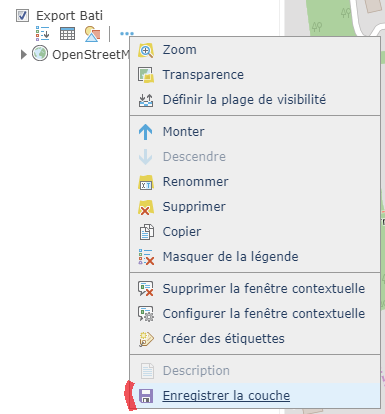
\includegraphics[width=0.4\textwidth]{img/cours3/ago_enregistrer_couche.png} \\
\end{figure}

\action Dans la fenêtre \textbf{Créer un élément}, conservez le titre (\textit{Export\_Bati}), ajoutez une balise \textit{ENSG} qui aidera les utilisateurs à trouver la carte lors de leurs recherches, puis cliquez sur \textbf{Créer un élément}.

Nous utiliserons ensuite un générateur d'application web intégré à ArcGIS Online pour produire le squelette de notre application web SIG.

\action Dans vos contenus sur ArcGIS Online, sélectionnez la carte \textit{BATI\_DESCARTES}.

\action Cliquez sur \textbf{Créer une application web > Utilisation d'un modèle}.
\begin{figure}[H]
	\center 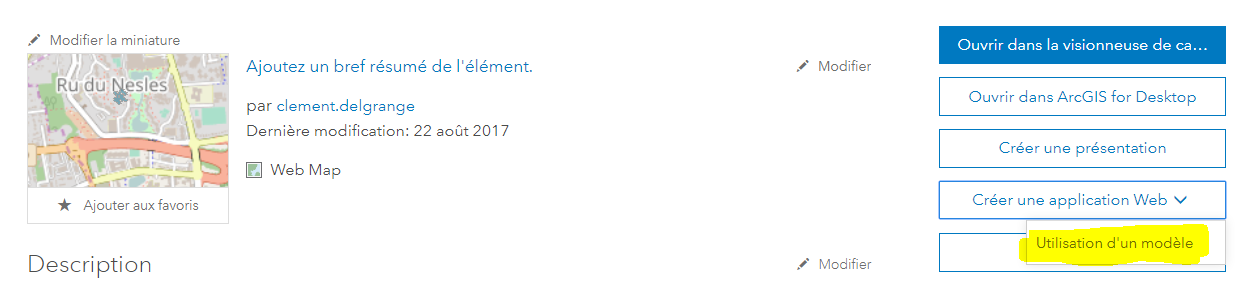
\includegraphics[width=0.7\textwidth]{img/cours3/ago_creer_appli_web.png} \\
\end{figure}

\action Plusieurs modèles d'application vous sont proposés : choisissez l'un des modèles de la catégorie \textbf{Présenter une carte}.

\action Cliquez sur \textbf{Créer une application web} et conservez les paramètres (nom, balises...) qui vous sont proposés.

\action Explorez les possibilités de personnalisation qui vous sont proposées : titre, couleurs, légende, widgets, etc.). Cliquez sur le bouton \textbf{Enregistrer} pour mettre à jour l'affichage en fonction de ce que vous avez modifié.

\action Lorsque vous avez terminé, cliquez sur \textbf{Fermer} pour générer le site web.

\action Il ne vous reste plus qu'à partager l'application pour la rendre visible par l'ensemble des utilisateurs.

Après avoir constaté que les applications de vos camarades sont bien visibles de tous, retournez sur votre application et ouvrez le code source de la page.

\action Sur quelle API l'application web est-elle basée et avec quelle API consomme-t-elle les services d’ArcGIS Online ?

\reponse





%\section{Utilisation d'ArcGIS Entreprise}
%\begin{note}
%ArcGIS Entreprise est la solution de serveur SIG d'Esri. Il s'agit du nouveau nom d'ArcGIS for Server, qui avait remplacé ArcIMS.
%\end{note}
%
%\subsection{Création de services dans ArcMap}
%Nous allons maintenant créer un service de carte afin de le publier sur un serveur ArcGIS. Un service de carte expose les informations contenues dans un document ArcMap (=le mxd).
%
%Pour commencer, nous allons connecter ArcMap au server ArcGIS de l'ENSG (zebra.ensg.eu).
%
%\action Dans le catalogue \textbf{> Serveurs SIG}, cliquez sur \textbf{Ajouter un serveur ArcGIS}.
%\begin{figure}[H]
%	\center 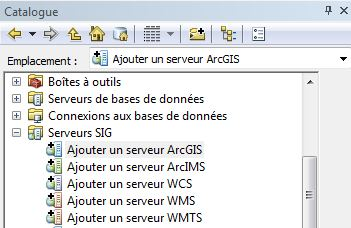
\includegraphics{img/cours3/am_ajouter_serveur_arcgis.jpg} \\
%\end{figure}
%
%\action Nous souhaitons pour l'instant publier de nouvelles ressources sur le serveur (\textit{publier les services GIS})
%\begin{figure}[H]
%	\center 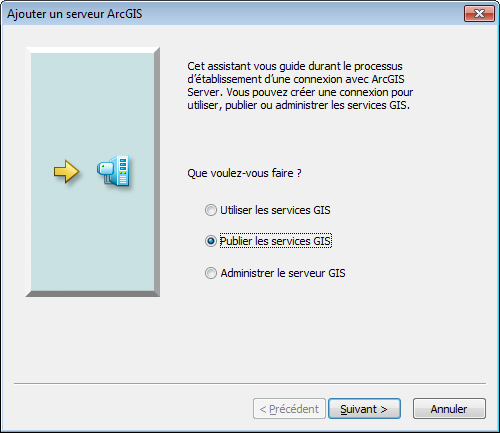
\includegraphics[width=0.5\textwidth]{img/cours3/am_ajouter_serveur_arcgis-2.png} \\
%\end{figure}
%
%\action Utilisez les paramètres ci-dessous :
%\begin{itemize}
%	\item URL : http://zebra.ensg.eu:6080/arcgis
%	\item Utilisateur : ing15
%	\item Mot de passe : ing15
%\end{itemize}
%
%\begin{figure}[H]
%	\center 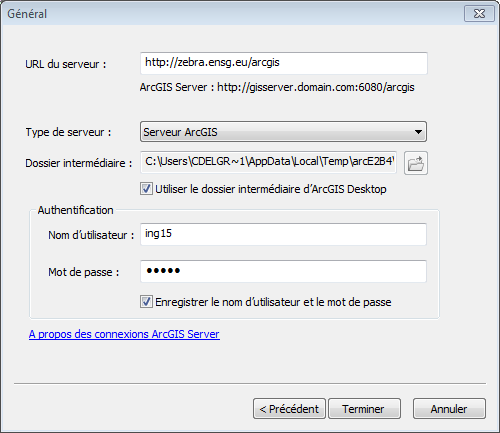
\includegraphics[width=0.5\textwidth]{img/cours3/am_connexion_serveur_arcgis.png} \\
%\end{figure}
%
%Lorsque vous validez, le serveur zebra.ensg.eu apparaît dans la liste des serveurs.
%\begin{figure}[H]
%	\center 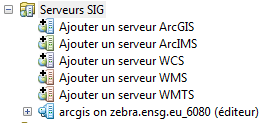
\includegraphics{img/cours3/am_connexion_ok_serveur_arcgis.png} \\
%\end{figure}
%
%Il ne nous reste plus qu'à publier le service.
%
%\action Allez dans le menu \textbf{Fichier > Partager en tant que > Service} pour commencer le paramétrage.
%
%Deux options s'offrent à l'utilisateur souhaitant créer un nouveau service :
%\begin{enumerate}
%	\item créer un fichier de définition de service qui sera ensuite lu par le serveur;
%	\item publier directement le service sur le serveur.
%\end{enumerate}
%
%La deuxième méthode revient en fait à enchaîner la création du fichier de définition du service et la lecture du fichier de définition par le serveur. Aussi afin de prendre le temps de bien comprendre toutes les étapes de la création d'un service nous passerons par le création d'un fichier de définition :
%
%\action Choisissez \textit{Enregistrer un fichier de définition de service}.
%\begin{figure}[H]
%	\center 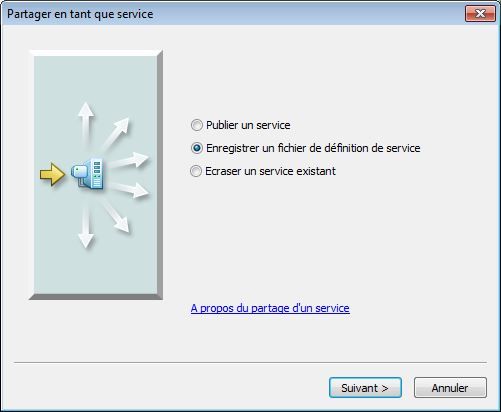
\includegraphics[width=0.4\textwidth]{img/cours3/am_publier_sd-1.jpg} \\
%\end{figure}
%
%\action Dans la fenêtre suivante, sélectionnez la connexion au serveur ArcGIS de l'ENSG (\textit{arcgis on zebra.ensg.eu\_6080}) et nommez votre service TD1\_<votre nom> :
%\begin{figure}[H]
%	\center 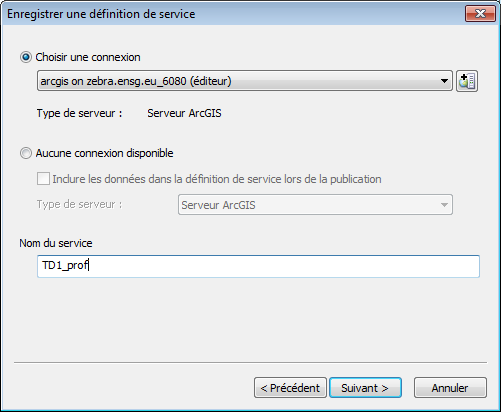
\includegraphics[width=0.4\textwidth]{img/cours3/am_publier_sd-2.png} \\
%\end{figure}
%
%\action Choisissez de publier le service dans le dossier existant du nom de votre groupe \textit{Ing15-gr1} ou \textit{Ing15-gr2} :
%\begin{figure}[H]
%	\center 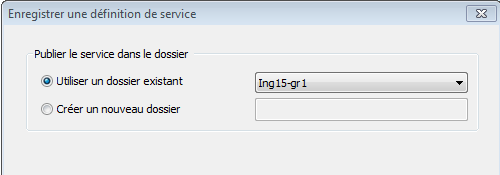
\includegraphics[width=0.4\textwidth]{img/cours3/am_publier_sd-3.png} \\
%\end{figure}
%
%\action Indiquez ensuite le répertoire de travail, sur votre disque, où vous enregistrerez le fichier de définition de service :
%\begin{figure}[H]
%	\center 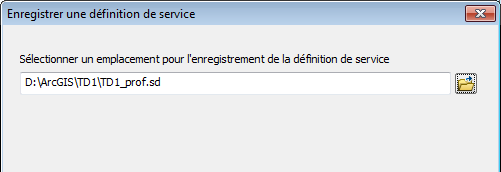
\includegraphics[width=0.4\textwidth]{img/cours3/am_publier_sd-4.png} \\
%\end{figure}
%
%Une fenêtre \textbf{Editeur de services} permet alors de paramétrer le service. Deux items nous intéresseront particulièrement :
%\begin{itemize}
%	\item \textbf{Fonctionnalités} qui permet de choisir les fonctionnalités du service à publier. \\
%	\action Choisissez les fonctionnalités \textit{Cartographie} et \textit{Feature Access}.
%	\item \textbf{Analyse} qui permet de s'assurer que la carte que nous souhaitons publier ne présente pas d'erreur.\\
%	\action Lancez l'analyse de votre document et corrigez les erreurs s'il y en a en vous aidant du descriptif ou de la proposition de correction.
%\end{itemize}
%
%\begin{figure}[H]
%	\center 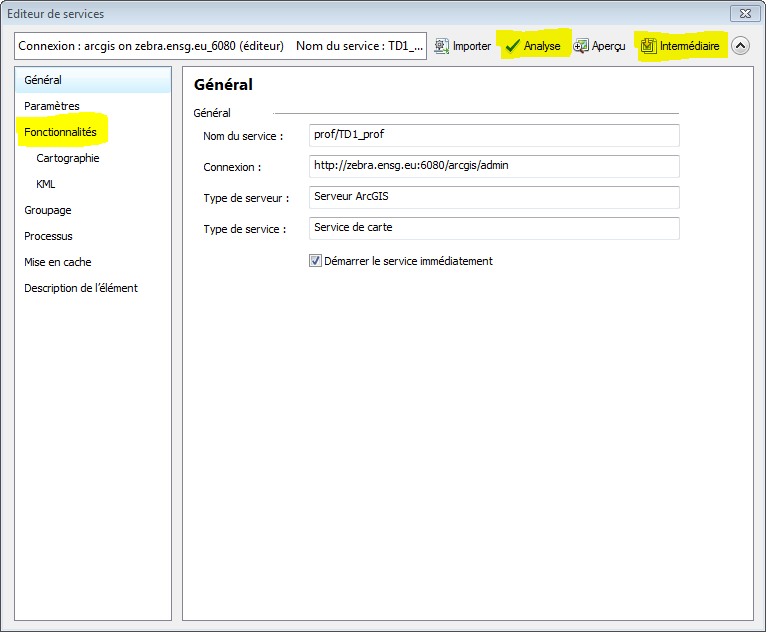
\includegraphics[width=0.7\textwidth]{img/cours3/am_publier_sd_parametrage.png} \\
%\end{figure}
%
%Lorsque votre document ne présente plus d'erreur et que le service est correctement configuré, vous pouvez lancer la génération du fichier de définition de service.
%
%\action Cliquez sur le bouton \textbf{Intermédiaire}.
%
%Il reste maintenant à publier le service sur le serveur.
%
%\action dans le catalogue d'ArcMap, identifiez le fichier de configuration (\textit{TD1\_<votre nom>.sd}.
%\begin{figure}[H]
%	\center 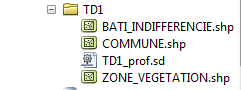
\includegraphics{img/cours3/am_publier_sd-5.png} \\
%\end{figure}
%
%\action Effectuez un clic droit sur ce fichier et choisissez \textbf{Publier en tant que...}.
%
%
%\subsection{Administration des services}
%Dans cette partie, nous nous intéressons au service de carte précédemment publié et essayons de modifier certaines de ces propriétés.
%
%\action Dans ArcMap, allez dans le catalogue et dépliez l'arborescence du serveur SIG de l'ENSG.
%
%\action Identifiez le service que vous avez publié lors de la partie précédente.
%\begin{figure}[H]
%%	\center \includegraphics{img/cours3/am_service_ags.png} \\
%\end{figure}
%
%\action En effectuant un clic droit sur votre service, sélectionnez \textbf{Propriétés du service}.
%
%Cet action ouvre une fenêtre similaire à celle qui nous a permis de paramétrer le service avant de le publier. Il s'agit d'un premier moyen de modifier un service publié sur un ArcGIS serveur.
%
%\action Constatez que les deux fonctionnalités sélectionnées lors de la publication sont bien activées et notez leurs URLs REST.
%
%\reponse
%
%\begin{note}
%REST (Representational State Transfer) est un style d'architecture qui repose et sur le protocole HTTP et permet d'accéder à une ressource via une adresse unique.
%\end{note}
%
%Nous allons pour l'instant nous concentrer sur la fonctionnalité de cartographie du service de carte publié.
%
%\action Ouvrez l'URL REST de cette fonctionnalité dans un navigateur web puis visualisez le rendu en cliquant sur le lien \url{arcgis.com}.
%\begin{figure}[H]
%%	\center \includegraphics[width=0.7\textwidth]{img/cours3/am_service_url_rest.png} \\
%\end{figure}
%
%\action Observez ce qu'il est possible de faire avec ce service (navigation, consultation des attributs, modifications géométriques et/ou attributaires, etc.).
%
%\action Effectuez la même opération avec la fonctionnalité \textit{Feature Access} et notez les différences.
%
%\reponse
%
%Pour administrer un serveur ArcGIS, Esri met également à notre disposition une application, ArcGIS Server Manager, accessible depuis un navigateur web : \url{http://<servername>:6080/arcgis/manager}.
%
%\action En utilisant le manager d'ArcGIS serveur, activez la fonctionnalité WMS du service de carte publié en première partie de ce TP.
%
%\begin{note}
%Les possibilité d'administration, via l'API REST, d'un serveur ArcGIS ne se limitent pas à l'activation de fonctionnalités, mais couvrent l'ensemble des tâches d'administration d'un serveur SIG (gestion des utilisateurs, des droits et des accès, etc.).
%\end{note}


\end{document}
